\documentclass[12pt]{article}
\usepackage{parskip}
\usepackage{verbatim}
\usepackage{listings}
\usepackage{epsfig}
\usepackage{tabularx}
\usepackage{graphicx}
\usepackage{caption}
\usepackage{subcaption}
\usepackage[margin=2cm]{geometry}

\title{COSC441 --- Assignment 1 and 2}
\author{Edward Hills}
\date{}

\begin{document}
\vspace{-1cm}

\maketitle

\section*{Assignment 1}

Here is a brief overview of my system.

\texttt{master.c} is the main thread and is responsible for creating and initialising the POSIX \texttt{pthreads} used to represent discs in the system and the worker threads. Once the discs and workers have been created, the workers will send a series of READ and WRITE requests for the discs to process. Once all requests have been processed the worker threads will quit and the master thread will send a QUIT message to each disc, once received the discs will also exit.-
Each disc thread has has been set up to have two message queues, one for WRITE requests and one for READ requests. These have been implemented as circular buffers. The disc thread will then poll each queue for a message to process. Each message will contain a READ/WRITE/QUIT flag and a pointer to a monitor.

A monitor will contain a series of information needed to process the request. Once it has been processed a flag will be set informing the relevant worker thread it has completed. I tried to use \texttt{pthread\_cond\_wait(3)} and \texttt{pthread\_cond\_signal(3)} to signal the worker thread responsible for accepting the reply from the latest disc request. This however introduced a dead-lock I was unable to track down.

After using \texttt{gprof} I found that the loop that checks for new requests is a major bottleneck also, however because I have two message queues, it is not possible to use signalling and wait here. \texttt{sched\_yield(2)} did make a large increase in performance however. Although, for smaller jobs or a computer with more CPU cores (I currently have two) it may not be as effective as the scheduler is unable to schedule the thread back in fast enough.

Seeing as I use a very simple circular buffer to store my messages, one for WRITE messages and one for READ messages, I could have had the disc access the queues without needing a lock. The reason a lock would not be needed is that the only race-condition that could occur is when a worker thread wanting to write the message finds that the queue is full (when it actually is not), in this case it is not important as it will check again when it is scheduled back into the CPU. The disc is the able to read the queue without causing interference of the worker thread writing to the queue. The difference in execution-time between the disc locking the queue and not locking the queue turns out to be negligible.

To be perfectly honest, I still never fully understood how the buffer rings was suppose to work. I realised that we should not write actual bytes (although I do memset a couple of buffers, just for fun), but I am not sure on how we were suppose to implement the read-ahead, write-behind buffers. Also an area of confusion I had, was the read when its full, write when its empty business.

To me a message passing system would have been far more elegant.

\section*{Assignment 2}

If Assignment 1 had been implemented with a message-passing system instead of using shared memory, I believe that it would have been easier to maintain and develop. In essence, message-passing is where one process sends messages containing possibly complex data-structures to a series of recipients. Conceptually, this is not dissimilar to the approach taken in the first assignment, that is, a worker thread messages a disc with a request and a location to where it can find the data. In a message-passing system, instead of a pointer to shared-memory, it would be a copy of the data itself.

Message-passing is also quite different from having a shared message-queue which is effectively just a form of the above. A shared message-queue is usually implemented so that each message contains the process ID of the process that should read that message.

Using message-passing allows easier construction of an asynchronous system. This allows one process (or thread) to send a message to another without blocking, and then be messaged back at a later date with a reply. 

A possible solution to Assignment 1 using message-passing is the implementation of a TCP sliding-window protocol almost, if order of requests is important. The worker thread would store the information about what disc to read from / write to and the block number, \emph{etc.} as it does in the shared-memory implementation. It would then message the respective disc and then process other requests if it has any. 

Once the disc thread receives the message containing what to do and the information it needs, it would perform its duty and then send a message back to the worker thread containing any and all information required. This could be a completion-time and maybe the bytes read also. To maintain an order of requests, the worker thread would need to maintain a buffer of replies. Each reply would need to be numbered in a way so that it was possible to tell what order they should be in, much like the TCP protocol. Once all replies have been received for some particular task (perhaps the worker had to send five requests to read from a file) then the replies can be put in order and processed by the worker. Of course if the worker only needs one reply then this is not needed. 

By using message-passing we can avoid much of the time that is wasted by waiting for tasks to complete. For example, in Assignment 1, I have a loop that is either busy-waiting checking to see if the shared data-structure has been modified (or ideally it would be signalled). With message-passing, it would have to do no waiting and can instead be performing any other tasks required of it, including sending further requests it may have. This is because it will simply receive a message containing the information that has been processed, rather than having to pro-actively go and search for it.

An important difference to be noted with a message-passing implementation is that there would be no locking required. This can greatly improve system performance. Because the required resources, shared message queues, and the files themselves used in assignment 1 are shared, we must lock and protect each. In the message-passing system nothing will be shared and all resources will have an associated process with it. For example, the message queues that store the requests sent from a worker for a disc would not require a lock because the disc would instead receive a message, and then deal with it. The disc is in-charge of these resources and is not shared to outside threads.

In real systems, mapping files to memory is common. However, in a message-passing system, it is not possible map files as this is still a form of shared-memory.

A possible draw-back of message-passing is synchronisation that may be needed. In this assignment this is not an issue, however in a real system, where perhaps files were being moved around on disc (and therefore the blocks no longer valid), a message-passing system such as this would not work. As a worker would try to send a request to disc, by the time the disc got the request, the file or block may no longer be there. Having shared-memory would avoid this problem as the worker would be able to see the same information that the disc was currently holding.

To me, assignment 2 would not be implemented that differently from assignment 1. The major difference, in my implementation, would be the removal of shared memory and replaced with copies of the data. 

Here is a diagram showing an abstract view of the message-passing system:

\begin{figure}
\centering
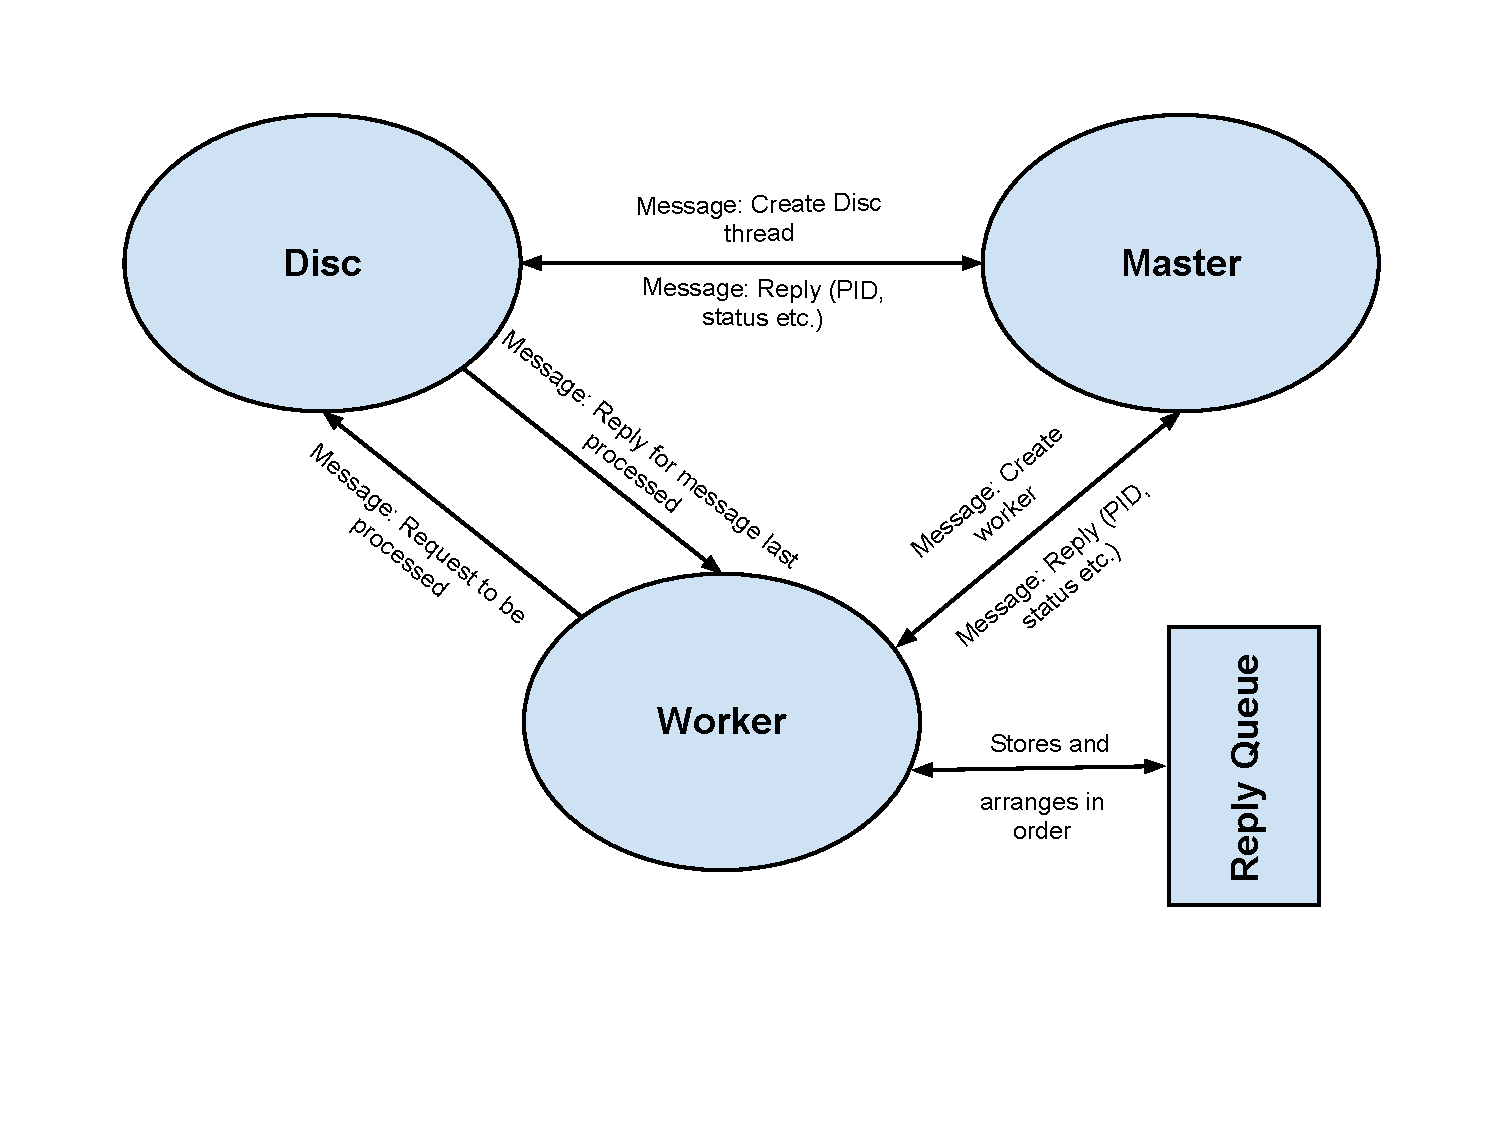
\includegraphics[width=18cm]{message-passing.pdf}
\caption{Abstract view of the message-passing implementation of Assignment 1}
\label{fig:message-passing}
\end{figure}

Making it message passing could help make asynchronisation easier. becasue can just og off and then be caled with data. would need to store a window of replies. in fact. it would be almost identical to the tcp sliding window protocol.

\end{document}
